\documentclass[../main.tex]{subfiles}
\begin{document}

% Figure 07: IAS2 Disc with Symington Surgeries
\begin{figure}[H]
    \centering
    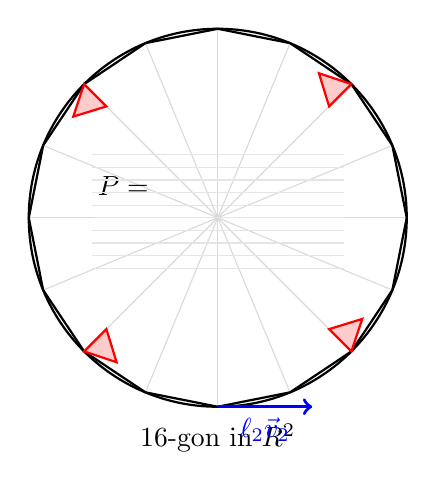
\begin{tikzpicture}[scale=0.8]
        % 16-gon background
        \draw[thick] (0,0) circle (3cm);
        \foreach \i in {0,22.5,...,337.5} {
            \draw[gray!30] (0,0) -- (\i:3cm);
        }
        
        % 16-gon boundary
        \foreach \i in {0,1,...,15} {
            \draw[thick] (\i*22.5:3cm) -- ({(\i+1)*22.5}:3cm);
        }

        % Labels
        \node at (0, -3.5) {16-gon in $\mathbb{R}^2$};
        \node at (-1.5, 0.5) {$P = $};

        % Symington Surgery Triangles (4 red triangles)
        \foreach \i in {45, 135, 225, 315} {
            \fill[red!20, draw=red, thick] (\i:3cm) -- (\i:2.5cm) -- (\i+10:2.8cm) -- cycle;
        }

        % Vectors
        \draw[->, blue, very thick] (0,-3) -- (1.5,-3) node[midway, below] {$\ell_2 \vec{v}_2$};
        
        % Interior Shading (representative)
        \foreach \i in {1,...,10} {
            \draw[gray!20] (-2, \i*0.2 - 1) -- (2, \i*0.2 - 1);
        }
    \end{tikzpicture}
    \caption{IAS2 Construction with Symington Surgeries.}
\end{figure}

% Figure 11: Geometric Degeneration (Triangulated Rectangle)
\begin{figure}[H]
    \centering
    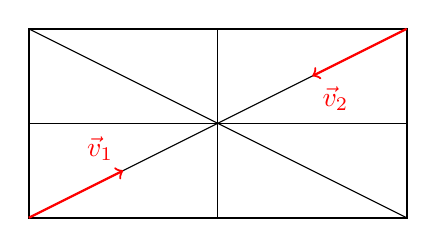
\begin{tikzpicture}[scale=1.2]
        \draw[thick] (0,0) rectangle (4,2);
        \draw (0,0) -- (4,2);
        \draw (0,2) -- (4,0);
        \draw (2,0) -- (2,2);
        \draw (0,1) -- (4,1);
        
        % Vectors pointing correctly
        \draw[->, thick, red] (0,0) -- (1, 0.5) node[above left] {$\vec{v}_1$};
        \draw[->, thick, red] (4,2) -- (3, 1.5) node[below right] {$\vec{v}_2$};
    \end{tikzpicture}
    \caption{Corrected Geometric Degeneration (Triangulated Rectangle).}
\end{figure}

% Figure 12: Stable Gluing (Hemisphere)
\begin{figure}[H]
    \centering
    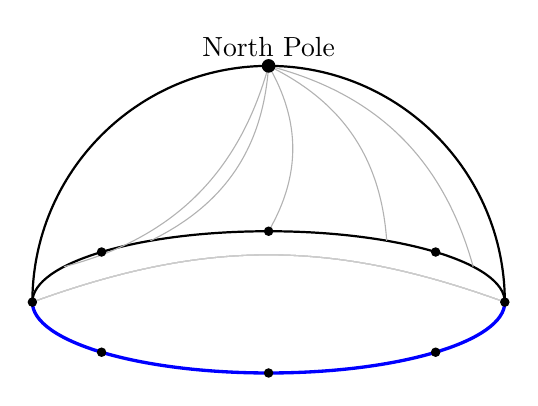
\begin{tikzpicture}[scale=1.5]
        % Hemisphere
        \draw[thick] (2,0) arc (0:180:2 and 0.6);
        \draw[thick, blue, very thick] (2,0) arc (0:-180:2 and 0.6); % Blue equator
        \draw[thick] (-2,0) arc (180:0:2 and 2);
        
        % Triangulation Arcs
        \foreach \i in {30,60,...,150} {
            \draw[gray!60] (0,2) to[bend left] (\i:2 and 0.6);
        }
        \foreach \i in {-0.6,-0.3,0,0.3,0.6} {
             \draw[gray!40] (-2,0) to[bend left=20] (2,0); % Representative arcs
        }

        % Nodes
        \filldraw[black] (0,2) circle (1.5pt) node[above] {North Pole};
        \foreach \i in {0,45,...,315} {
            \filldraw[black] ({2*cos(\i)}, {0.6*sin(\i)}) circle (1pt);
        }
    \end{tikzpicture}
    \caption{Stable Gluing: Hemisphere Triangulation with Blue Equator.}
\end{figure}

\end{document}
